\section{Descrizione dell'architettura}
\subsection{Architettura frontend}
\subsubsection{Design pattern architetturale}

\paragraph{Redux-Toolkit}
I componenti che costituiscono l’architettura frontend utilizzata seguono il pattern offerto dalla libreria Redux-
Toolkit.
Redux-Toolkit è pensato per integrarsi con React e il principale vantaggio che offre è quello di poter
gestire i dati condivisi tra i componenti React in modo centralizzato semplificando la gestione dello stato
globale dell’applicazione.
Inoltre Redux-Toolkit è un wrapper che semplifica l'utilizzo di Redux in modo tale da scrivere meno codice e commettere meno errori durante lo sviluppo.

I componenti che formano l’architettura di Redux-Toolkit sono:
\begin{itemize}
    \item \textbf{Store:} componente che contiene lo stato globale dell’applicazione.
    All’avvio dell’applicazione viene configurato utilizzando RootReducer e i componenti che utilizzano
    lo stato globale si mettono in ascolto dello store in modo da venire renderizzati ogni volta che un dato
    di interesse cambia valore. Questo modo di operare può essere visto come un pattern Observer in
    cui lo store è il Subject e gli Observer sono i componenti React che osservano i cambiamenti dello store;
    \item \textbf{RootReducer:} componente utilizzato per configurare lo store combinando le slice;
    \item \textbf{Slice:} componente che contiene un proprio stato che rappresenta una porzione dello stato globale
    dell’applicazione, i reducer che operano su tale stato e i selector per consentire ai suoi client il
    reperimento dei dati;
    \item \textbf{Reducer:} componente che riceve come parametri uno stato iniziale (InitialState) e un'action
    (composta da un type e un payload) e restituisce lo stato dopo aver operato sui dati. 
    Il type rappresenta una stringa univoca che ha lo scopo di identificare la specifica action che si intende eseguire.
    Il payload è un oggetto che contiene i dati necessari per l'esecuzione dell'action.
    React-Toolkit gestisce le chiamate ai reducer in seguito ai dispatch delle action che avvengono
    specificando solamente l’oggetto che rappresenta il payload;
    Con il termine dispatch si intende una funzione che viene chiamata per inviare una action allo store di Redux e innescare un cambiamento dello stato.
    \item \textbf{Action:} oggetto composto da un type e da un payload di cui viene effettuato il dispatch quando
    opportuno. Il payload è un oggetto che contiene i dati da passare al reducer che catturerà l’action;
    \item \textbf{InitialState:} componente che contiene i dati di una slice su cui essa opera.
    Importante sottolineare che Redux-Toolkit garantisce l’immutabilità dei dati in modo che i reducer restituiscano delle copie dello stato in modo che esso non possa venire
    modificato dall’esterno è utilizzato in modo improprio.
    L’unico modo per modificare i dati dello stato globale `e quindi con il dispatch di un’action;
    \item \textbf{Selector:} funzione che prende lo stato corrente di una slice come argomento e ritorna un sottoinsieme
    specifico del suo stato. In altre parole, un selector consente di selezionare una parte specifica
    dello stato in modo da poterla utilizzare in modo isolato all’interno di un componente React.
\end{itemize}

\subsubsection{Elenco dei componenti}
Poiché il team di sviluppo frontend utilizzerà Redux per la gestione dello stato, l'applicazione sarà strutturata principalmente attraverso la suddivisione del codice in slice, stati iniziali e action.
\paragraph{Slice}
    Le slice contengono una porzione dello stato globale dell’applicazione che è gestita da un reducer
    specifico.
\begin{itemize}
        \item \textbf{DataSlice:} componente che gestisce lo stato e contiene i dati relativi al dataset selezionato dall'utente;
        \item \textbf{AppStateSlice:} componente che gestisce lo stato dell'applicazione come errori e caricamenti;
        \item \textbf{DataSourceSlice:} componente che gestisce lo stato e contiene l'elenco dei dataset selezionabili dall'utente e il dataset selezionato;
        \item \textbf{FilterOptionSlice:} componente che gestisce lo stato e contiene le opzioni di filtraggio dei valori;
        \item \textbf{ViewOptionSlice:} componente che gestisce lo stato e contiene le opzioni di visibilità del piano medio;
        \item \textbf{RaycastHitSlice:} componente che gestisce lo stato e contiene le informazioni relative al raycast.
\end{itemize}
\paragraph{Initial state}
    Gli stati iniziali, definiti all'interno di ciascuna slice, si combinano per formare lo stato globale iniziale, gestito dallo store.
    \begin{itemize}
        \item \textbf{DataState:} componente che contiene i dati relativi al dateset selezionato dall'utente;
        \item \textbf{AppState:} componente che contiene i dati relativi allo stato attuale dell'applicazione;
        \item \textbf{DataSourceState:} componente che contiene le informazioni principali di tutti i dataset e quelle relative al dataset selezionato dall'utente;
        \item \textbf{FilterOptionState:} componente che contiene i dati relativi alle opzioni di filtraggio selezionate dall'utente;
        \item \textbf{ViewOptionState:} componente che contiene i dati relativi alle opzioni di visibilità del piano medio all'interno dell'ambiente 3D;
        \item \textbf{RaycastHitState:} componente che contiene i dati relativi al raycast, utilizzati per l'interazione con le barre del grafico 3D.
    \end{itemize}
\paragraph{Action}
    Le action, emesse dai componenti, vengono inviate ai reducer per aggiornare lo stato corrispondente.
    Ogni action è caratterizzata da un type e da un payload, che viene utilizzato dalle slice per modificare lo stato.
    Per convenzione il nome delle action segue il formato: \\
    \begin{center}
        \textbf{[nome slice dalla quale viene catturata].[nome action]}.
    \end{center}
    \begin{itemize}
        \item \textbf{DataSlice.requestData:} action asincrona emessa per recuperare dal server i dati del dataset selezionato; \\ Payload: nessuno
        \item \textbf{DataSlice.filterTopN:} action emessa per filtrare i dati, visualizzando esclusivamente i primi N valori più alti o più bassi; \\ Payload: FilterPayload
        \item \textbf{DataSlice.filterAboveValue:} action emessa per filtrare i dati, visualizzando esclusivamente quelli con un valore maggiore o minore rispetto al valore della barra del grafico selezionata;\\ Payload: FilterPayload
        \item \textbf{DataSlice.filterAverage:} action emessa per filtrare i dati, visualizzando esclusivamente quelli con un valore maggiore o minore rispetto alla media globale; \\ Payload: boolean $\rightarrow$ maggiore o minore
        \item \textbf{AppStateSlice.setLoading:} action emessa per aggiornare lo stato dell'applicazione e visualizzare la pagina di caricamento; \\ Payload: boolean
        \item \textbf{AppStateSlice.setError:} action emessa per aggiornare lo stato dell'applicazione e visualizzare una schermata di errore specifica, basata sull'errore generato dall'applicazione; \\ Payload: number $\rightarrow$ codice di errore.
        \item \textbf{DataSourceSlice.requestDatasets:} action asincrona emessa per recuperare l'elenco delle informazioni relative a tutti i dataset disponibili; \\ Payload: nessuno.
        \item \textbf{DataSourceSlice.setCurrentDataset:} action emessa per aggiornare il dataset selezionato dall'utente; \\ Payload: number $\rightarrow$ ID del dataset.
        \item \textbf{ViewOptionSlice.toggleAveragePlane:} action emessa per aggiornare il flag di visibilità del piano medio globale nell'ambiente 3D; \\ Payload: boolean 
        \item \textbf{FilterOptionSlice.toggleIsGreater:} action emessa per aggiornare il flag che determina se il filtraggio deve essere eseguito per valori maggiori o minori; \\ Payload: boolean
        \item \textbf{RaycastHitSlice.setHit:} action emessa per aggiornare la barra selezionata nel grafico 3D; \\ Payload: number $\rightarrow$ ID della barra.
        \item \textbf{RaycastHitSlice.setTooltipPosition:} action emessa per aggiornare la posizione del tooltip in base alla posizione del puntatore.\\ Payload: Vector3 $\rightarrow$ posizione del puntatore.
    \end{itemize}
\paragraph{Classi}
    Classi offerte dalle librerie utilizzate:
    \begin{itemize}
        \item \textbf{Vector3:} classe offerta dalla libreria Three.js. Rappresenta un vettore tridimensionale, ovvero
        una grandezza fisica caratterizzata da una direzione e da una lunghezza. Il vettore tridimensionale
        viene comunemente utilizzato per definire la posizione, la rotazione, la scala e la direzione
        delle barre del grafico 3D;
        \item \textbf{Provider:} Componente Redux che rende lo store accessibile a tutti i componenti dell'applicazione, "avvolgendo" il componente principale App e accettando lo store come prop;
        \item \textbf{Store:} Lo store Redux traccia lo stato dell'applicazione, contiene il reducer principale per la gestione delle action e fornisce metodi per accedere allo stato,
        registra i listener per le modifiche di stato;
        \item \textbf{RootReducer:} componente Redux che combina tutti i reducer dell’applicazione in uno stato
        globale. Questa funzione viene passata allo store per gestire lo stato complessivo dell’applicazione;
        \item \textbf{FontLoader:} classe utility di Three.js che permette di caricare dati di font in formato JSON per poi generare mesh di testo in ambienti tridimensionali;
        \item \textbf{Gsap:} classe utility della libreria gsap che permette di creare animazioni sia dell'interfaccia utente (UI) e sia all'interno dell'ambiente 3D con facilità e poco codice.
        \item \textbf{Canvas:} componente React Three Fiber che comprende gli elementi grafici che vanno a costituire la scena 3D. 
        Fornisce una telecamera e una scena con una serie di props opzionali utili alla configurazione dell’ambiente 3D;
        \item \textbf{OrbitControls:} componente React Three Fiber che abilita la navigazione e la manipolazione della telecamera utilizzando gli input del mouse;
    \end{itemize}
    Classi definite dal team:
    \begin{itemize}
        \item \textbf{Dataset:} classe che rappresenta l'intero dataset con relative etichette e legenda;
        \item \textbf{Legend:} classe che rappresenta la legenda del dataset selezionato;
        \item \textbf{Data:} classe che rappresenta un singolo dato, visualizzato come una barra nel grafico;
        \item \textbf{AppState:} classe che rappresenta lo stato globale dell'applicazione;
        \item \textbf{DatasetInfo:} classe che rappresenta un dataset e ne memorizza le informazioni principali;
        \item \textbf{RaycastHit:} classe che rappresenta il punto di intersezione tra il puntatore e una barra del grafico;
        \item \textbf{FilterPayload:} classe che rappresenta il payload da inviare alle action di filtraggio del DataSlice;
        \item \textbf{MaxRequestError:} classe che rappresenta un errore di superamento del limite massimo di richieste effettuate;
        \item \textbf{NetworkError:} classe che rappresenta un errore di comunicazione e connessione alle API;
        \item \textbf{ServerError:} classe che rappresenta un errore di connessione al server.
    \end{itemize}
\paragraph{Componenti React UI}
    I seguenti componenti, sviluppati dal team, visualizzano i dati dello stato che compongono la UI:
    \begin{itemize}
        \item \textbf{ErrorPage:} componente che visualizza la pagina di errore dell'applicazione;
        \item \textbf{HomePage:} componente che visualizza la homepage dell'applicazione;
        \item \textbf{DatasetItem:} componente che visualizza i metadati di un dataset.
        \item \textbf{UI:} componente che aggrega i componenti grafici che compongono l'interfaccia utente;
                \item \textbf{Tooltip:} componente che visualizza un tooltip con i dettagli di una barra;
        \item \textbf{DataTable:} componente che visualizza una tabella contenente tutti i valori del dataset selezionato;
        \item \textbf{FilterModOption:} componente per la configurazione del tipo di filtraggio dati;
        \item \textbf{AveragePlaneOption:} componente per la selezione della visibilità del piano medio;
        \item \textbf{NFilter:} componente che consente l'inserimento di un valore N e applica il filtraggio ai primi N valori più alti o più bassi;
        \item \textbf{Filter:} componente che implementa un filtro generico capace di filtrare valori superiori o inferiori rispetto a un dato valore di riferimento;
    \end{itemize}
\paragraph{Componenti tridimensionali di Three.js}
    I seguenti componenti visualizzano i dati del dataset all'interno dell'ambiente 3D tramite un grafico.
    \begin{itemize}
        \item \textbf{EnvironmentPage:} componente che permette di visualizzare la pagina in cui viene renderizzato l'ambiente 3D;
        \item \textbf{CustomCanvas:} componente che fornisce una telecamera e una scena tridimensionale, configurabili tramite props opzionali;
        \item \textbf{BarChart:} componente che permette di visualizzare un grafico 3D;
        \item \textbf{AveragePlane:} componente che permette di visualizzare il piano medio globale;
        \item \textbf{Bars:} componente che permette di visualizzare una singola barra in un grafico 3D;
        \item \textbf{Raycaster:} componente che gestisce la logica di intersezione tra il puntatore e le barre del grafico;
        \item \textbf{ZAxis:} componente che rappresenta l'asse Z del grafico 3D;
        \item \textbf{XAxis:} componente che rappresenta l'asse X del grafico 3D;
        \item \textbf{YAxis:} componente che rappresenta l'asse Y del grafico 3D;
        \item \textbf{Lights:} componente che gestisce l'illuminazione all'interno della scena tridimensionale.
    \end{itemize}

\pagebreak

\subsubsection{Architettura logica}
I diagrammi delle classi sono organizzati per slice e componenti React per una lettura più semplice. 
Sono presenti anche diagrammi che mostrano le dipendenze generali tra i componenti React.\\\\
\textbf{Nota:}\\
I rettangoli che rappresentano le classi sono colorati per distinguere i diversi tipi di componenti.
\begin{itemize}
    \item \textbf{Bianco:} normali classi;
    \item \textbf{Giallo:} action di Redux;
    \item \textbf{Blu:} componenti React.
\end{itemize}

\paragraph{DataSlice}
\begin{figure}[h!] \centering
    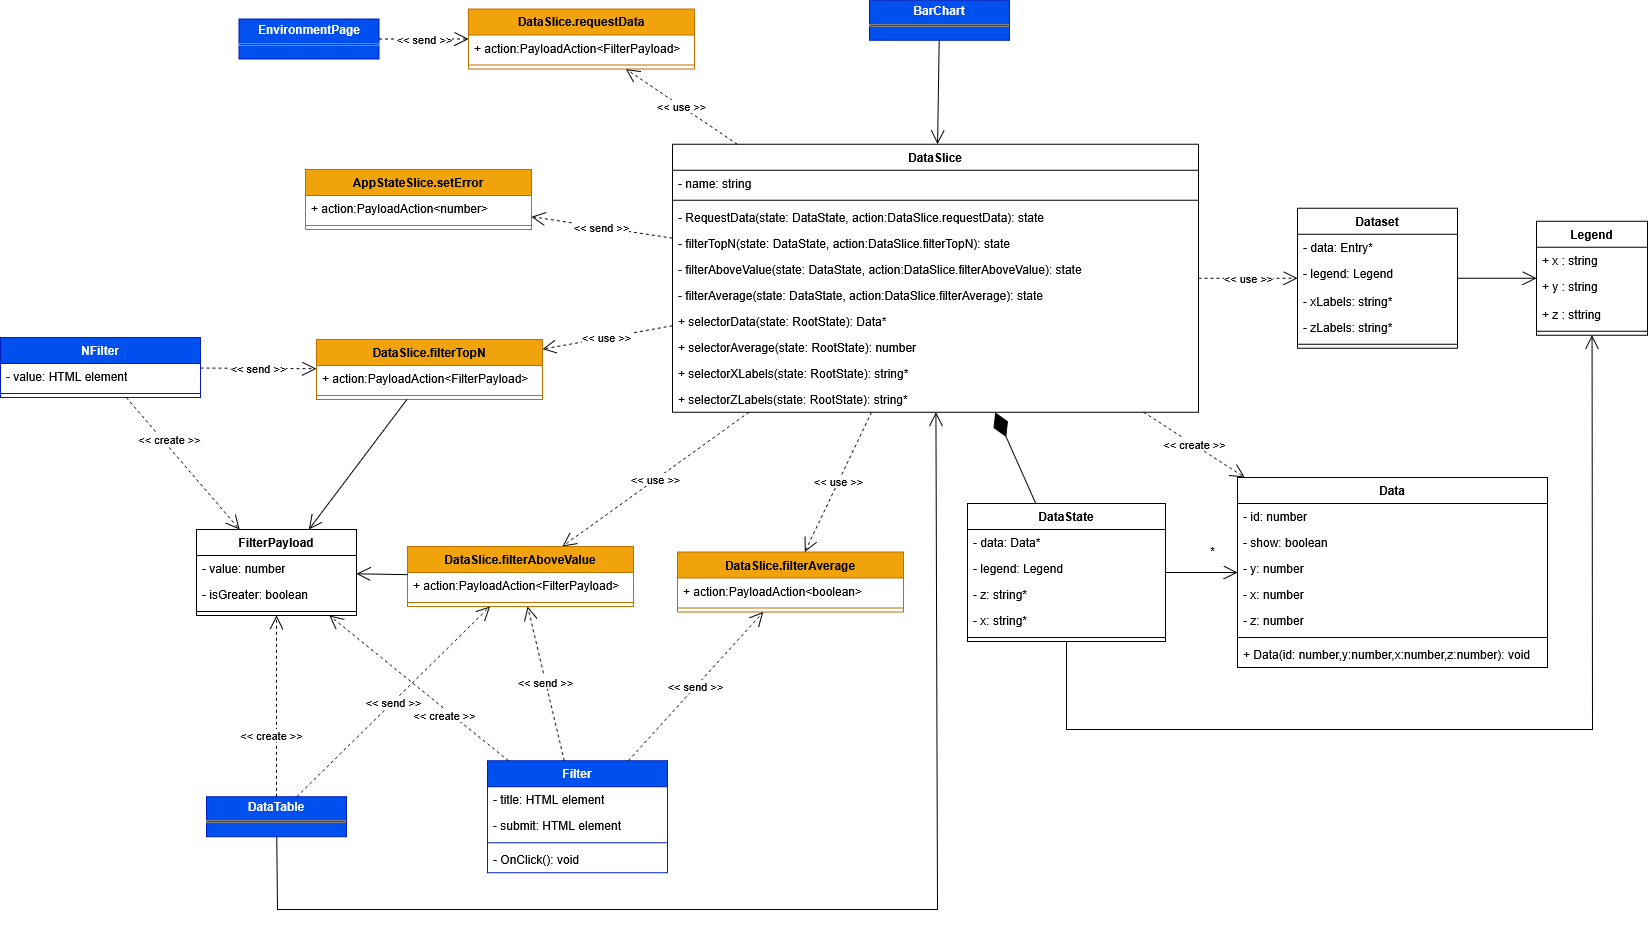
\includegraphics[scale=0.3]{template/images/uml_front/logic/dataslice.png}
    \caption{DataSlice}
\end{figure}
\textbf{Descrizione del diagramma:}\\
Questo diagramma include tutti i componenti utili per recuperare e filtrare i dati provenienti dal server.
\begin{itemize}
    \item \textbf{DataSlice:}
    \begin{itemize}
        \item \textbf{Dipendenze:}
        \begin{itemize}
            \item DataState (composizione): gestisce la creazione e la distruzione dell'istanza di DataState, che non è condivisa con altri componenti;
            \item RawData (dipendenza semplice <<use>>): rappresenta una singola entry del dataset;
            \item Data (dipendenza semplice <<create>>): responsabile della creazione dei singoli oggetti Data che verranno inseriti nella lista di dati di DataState;
            \item DataSlice.requestData (dipendenza semplice <<use>>): cattura un'istanza di DataSlice.requestData e il reducer manda una richiesta al server per prendere i dati del dataset selezionato utilizzando il payload;
            \item DataSlice.filterTopN (dipendenza semplice <<use>>): cattura un'istanza di DataSlice.filterTopN e il reducer applica un filtro sui primi N valori più alti o più bassi, basandosi sui parametri di FilterPayload;
            \item DataSlice.filterAverage (dipendenza semplice <<use>>): cattura un’istanza di DataSlice.filterAverage e il reducer applica un filtro sui valori maggiori o minori rispetto alla media globale, basandosi sui parametri di FilterPayload;
            \item DataSlice.filterAboveValue (dipendenza semplice <<use>>): cattura un’istanza di DataSlice.filterAboveValue e il reducer applica un filtro sui valori maggiori o minori rispetto al valore della barra del grafico 3D selezionata, basandosi sui parametri di FilterPayload;
            \item AppStateSlice.setError (dipendenza semplice <<send>>): crea ed emette un’istanza dell’azione AppStateSlice.setError.
        \end{itemize} 
        \item \textbf{Interazioni:}
        \begin{itemize}
            \item DataState: viene modificato in base alle action catturate dal reducer della slice.
        \end{itemize} 
        \item \textbf{Action catturate:}
        \begin{itemize}
            \item DataSlice.filterTopN;
            \item DataSlice.filterAverage;
            \item DataSlice.filterAboveValue.
        \end{itemize} 
        \item \textbf{Action emesse:}
        \begin{itemize}
            \item AppStateSlice.setError.
        \end{itemize} 
    \end{itemize}

    \item \textbf{DataState:}
    \begin{itemize}
        \item \textbf{Dipendenze:}
        \begin{itemize}
            \item Data (associazione): contiene la lista dei dati del dataset.
            \item Legend (associazione): contiene la legenda del dataset.
        \end{itemize} 
    \end{itemize}

    \item \textbf{Dataset:}
    \begin{itemize}
        \item \textbf{Dipendenze:}
        \begin{itemize}
            \item Legend (associazione): contiene la legenda del dataset.
        \end{itemize} 
    \end{itemize}

    \item \textbf{NFilter:}
    \begin{itemize}
        \item \textbf{Dipendenze:}
        \begin{itemize}
            \item DataSlice.filterTopN (dipendenza semplice <<send>>): crea ed emette un’istanza dell’azione DataSlice.filterTopN;
            \item FilterPayload (dipendenza semplice <<create>>): responsabile della creazione dei payload di tipo FilterPayload che verranno poi utilizzati per applicare un filtro nel modo corretto.
        \end{itemize} 
        \item \textbf{Action emesse:}
        \begin{itemize}
            \item DataSlice.filterTopN;
        \end{itemize} 
    \end{itemize}

    \item \textbf{Filter:}
    \begin{itemize}
        \item \textbf{Dipendenze:}
        \begin{itemize}
            \item DataSlice.filterAverage (dipendenza semplice <<send>>): crea ed emette un’istanza dell’azione DataSlice.filterAverage;
            \item DataSlice.filterAboveValue (dipendenza semplice <<send>>): crea ed emette un’istanza dell’azione DataSlice.filterAboveValue;
            \item FilterPayload (dipendenza semplice <<create>>): responsabile della creazione dei payload di tipo FilterPayload che verranno poi utilizzati per applicare un filtro nel modo corretto.
        \end{itemize} 
        \item \textbf{Action emesse:}
        \begin{itemize}
            \item DataSlice.filterAverage;
            \item DataSlice.filterAboveValue.
        \end{itemize} 
    \end{itemize}

    \item \textbf{DataTable:}
    \begin{itemize}
        \item \textbf{Dipendenze:}
        \begin{itemize}
            \item DataSlice (associazione): contiene implicitamente un'istanza di DataSlice;
            \item DataSlice.filterAboveValue (dipendenza semplice <<send>>): crea ed emette un’istanza dell’azione DataSlice.DataSlice;
            \item FilterPayload (dipendenza semplice <<create>>): responsabile della creazione dei payload di tipo FilterPayload che verranno poi utilizzati per applicare un filtro nel modo corretto.
        \end{itemize} 
        \item \textbf{Interazioni:}
        \begin{itemize}
            \item DataSlice: vengono utilizzati i metodi selectorData,selectorXLabels e selectorZLabel per reperire la lista dei dati e delle etichette.
        \end{itemize} 
        \item \textbf{Action emesse:}
        \begin{itemize}
            \item DataSlice.filterAboveValue.
        \end{itemize} 
    \end{itemize}

    \item \textbf{BarChart:}
    \begin{itemize}
        \item \textbf{Dipendenze:}
        \begin{itemize}
            \item DataSlice (associazione): contiene implicitamente un'istanza di DataSlice.
        \end{itemize} 
        \item \textbf{Interazioni:}
        \begin{itemize}
            \item DataSlice: vengono utilizzati i metodi selectorData,selectorXLabels e selectorZLabel per reperire la lista dei dati e delle etichette.
        \end{itemize} 
    \end{itemize}

    \item \textbf{EnvironmentPage:}
    \begin{itemize}
        \item \textbf{Dipendenze:}
        \begin{itemize}
            \item DataSlice.requestData (dipendenza semplice <<send>>): crea ed emette un’istanza dell’azione DataSlice.requestData.
        \end{itemize} 
        \item \textbf{Action emesse:}
        \begin{itemize}
            \item DataSlice.requestData.
        \end{itemize} 
    \end{itemize}
\end{itemize}

\pagebreak

\paragraph{DataSourceSlice}
\begin{figure}[h!] \centering
    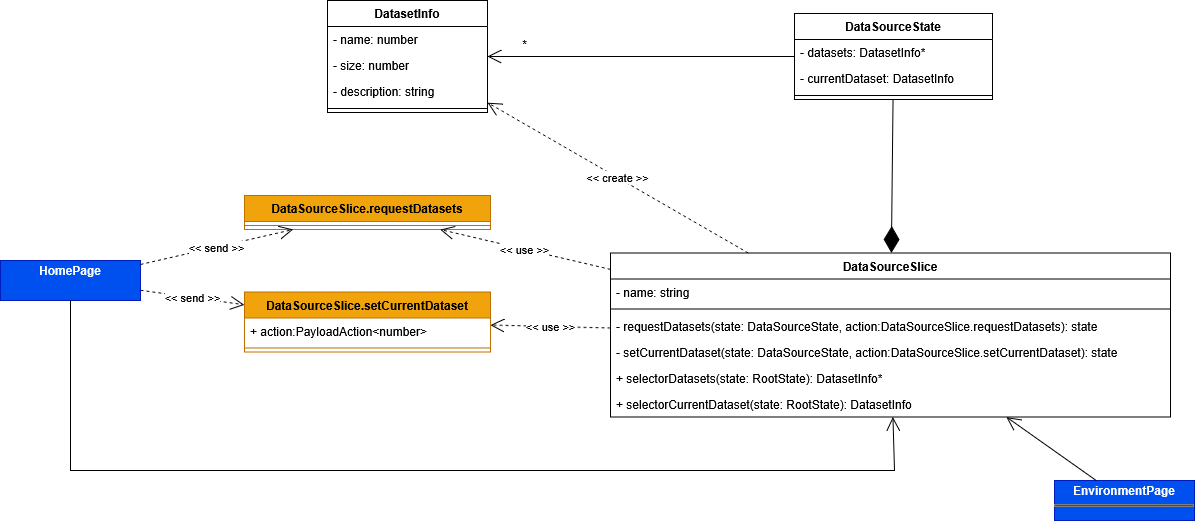
\includegraphics[scale=0.35]{template/images/uml_front/logic/datasourceslice.png}
    \caption{DataSourceSlice}
\end{figure}
\textbf{Descrizione del diagramma:}\\
Questo diagramma illustra i componenti per recuperare le informazioni chiave dai dataset proposti.
\begin{itemize}
    \item \textbf{DataSourceSlice:}
    \begin{itemize}
        \item \textbf{Dipendenze:}
        \begin{itemize}
            \item DataSourceState (composizione): gestisce la creazione e la distruzione dell'istanza di DataSourceState, che non è condivisa con altri componenti;
            \item DatasetInfo (dipendenza semplice <<create>>): responsabile della creazione dei singoli oggetti DatasetInfo che verranno inseriti nella lista di dataset di DataSourceState;
            \item DataSourceSlice.requestData (dipendenza semplice <<use>>): cattura un'istanza di DataSourceSlice.requestData e il reducer manda una richiesta al server per prendere la lista dei dataset e le loro principali informazioni;
            \item DataSourceSlice.setCurrentDataset (dipendenza semplice <<use>>): cattura un'istanza di DataSourceSlice.setCurrentDataset e il reducer ne utilizza il payload per aggiornare il dataset selezionato dall'utente.
        \end{itemize} 
        \item \textbf{Interazioni:}
        \begin{itemize}
            \item DataSourceState: viene modificato in base alle action catturate dal reducer della slice.
        \end{itemize} 
        \item \textbf{Action catturate:}
        \begin{itemize}
            \item DataSourceSlice.setCurrentDataset;
            \item DataSourceSlice.setCurrentDataset.
        \end{itemize} 
    \end{itemize}

    
    \item \textbf{DataSourceState:}
    \begin{itemize}
        \item \textbf{Dipendenze:}
        \begin{itemize}
            \item DatasetInfo (associazione): contiene la lista dei dataset proposti, con le loro informazioni, e quello corrente.
        \end{itemize} 
    \end{itemize}

    \item \textbf{HomePage:}
    \begin{itemize}
        \item \textbf{Dipendenze:}
        \begin{itemize}
            \item DataSourceSlice (associazione): contiene implicitamente un'istanza di DataSourceSlice;
            \item DataLabelSlice.requestData (dipendenza semplice <<send>>): crea ed emette un’istanza dell’azione DataLabelSlice.requestData;
            \item DataLabelSlice.setCurrentDataset (dipendenza semplice <<send>>): crea ed emette un’istanza dell’azione DataLabelSlice.setCurrentDataset.
        \end{itemize} 
        \item \textbf{Interazioni:}
        \begin{itemize}
            \item DataSourceSlice: viene utilizzato il metodo selectorDatasets per reperire la lista dei dataset.
        \end{itemize} 
        \item \textbf{Action emesse:}
        \begin{itemize}
            \item DataLabelSlice.requestData;
            \item DataLabelSlice.setCurrentDataset.
        \end{itemize} 
    \end{itemize}

    \item \textbf{EnvironmentPage:}
    \begin{itemize}
        \item \textbf{Dipendenze:}
        \begin{itemize}
            \item DataSourceSlice (associazione): contiene implicitamente un'istanza di DataSourceSlice.
        \end{itemize} 
        \item \textbf{Interazioni:}
        \begin{itemize}
            \item DataSourceSlice: viene utilizzato il metodo selectorCurrentDataset per reperire il dataset selezionato dall'utente e le sue informazioni.
        \end{itemize}  
    \end{itemize}
\end{itemize}

\paragraph{AppStateSlice}
\begin{figure}[h!] \centering
    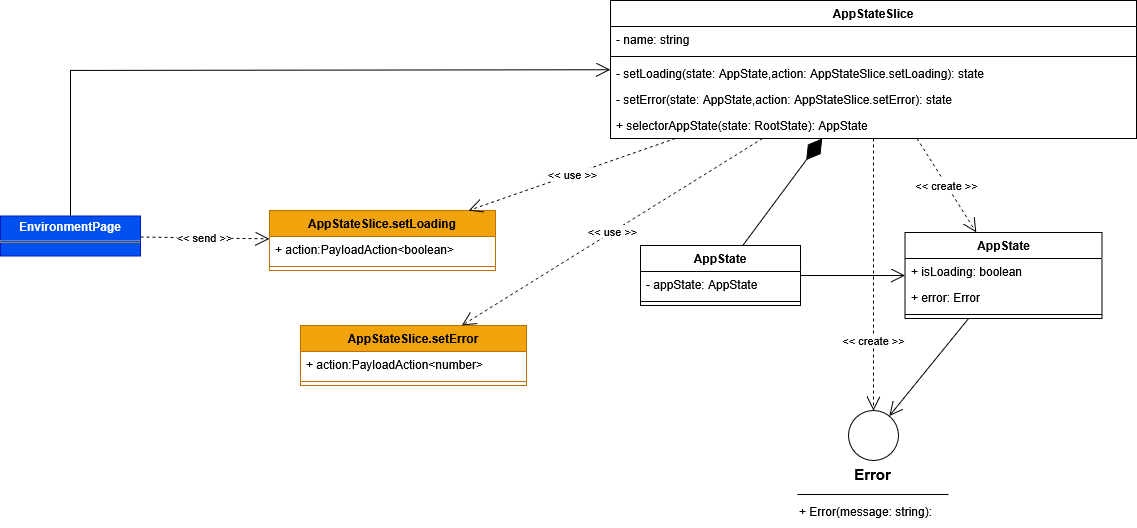
\includegraphics[scale=0.4]{template/images/uml_front/logic/appstateslice.png}
    \caption{AppStateSlice}
\end{figure}
\textbf{Descrizione del diagramma:}\\
Questo diagramma mostra i componenti per la gestione dello stato dell'applicazione.
\begin{itemize}
    \item \textbf{AppStateSlice:}
    \begin{itemize}
        \item \textbf{Dipendenze:}
        \begin{itemize}
            \item AppState (composizione): gestisce la creazione e la distruzione dell'istanza di AppState, che non è condivisa con altri componenti;
            \item AppState (dipendenza semplice <<create>>): responsabile della costruzione dell' oggetto AppState inserire all’interno dell AppState;
            \item AppStateSlice.setLoading (dipendenza semplice <<use>>): cattura un’istanza di AppStateSlice.setLoading e il reducer aggiorna lo stato di caricamento dell'applicazione utilizzando il payload;
            \item AppStateSlice.setError (dipendenza semplice <<use>>): cattura un’istanza di AppStateSlice.setError e il reducer aggiorna lo stato di errore dell'applicazione ne utilizza il payload.
        \end{itemize} 
        \item \textbf{Interazioni:}
        \begin{itemize}
            \item DataSourceState: viene modificato in base alle action catturate dal reducer della slice.
        \end{itemize} 
        \item \textbf{Action catturate:}
        \begin{itemize}
            \item AppStateSlice.setLoading;
            \item AppStateSlice.setError.
        \end{itemize} 
    \end{itemize}

    
    \item \textbf{AppState:}
    \begin{itemize}
        \item \textbf{Dipendenze:}
        \begin{itemize}
            \item AppState (associazione): contiene l'oggetto che rappresenta lo stato dell'applicazione.
        \end{itemize} 
    \end{itemize}

    \item \textbf{EnvironmentPage:}
    \begin{itemize}
        \item \textbf{Dipendenze:}
        \begin{itemize}
            \item AppStateSlice (associazione): contiene implicitamente un'istanza di AppStateSlice;
            \item AppStateSlice.setLoading (dipendenza semplice <<send>>): crea ed emette un’istanza dell’azione AppStateSlice.setLoading.
        \end{itemize} 
        \item \textbf{Interazioni:}
        \begin{itemize}
            \item AppStateSlice: viene utilizzato il metodo selectorAppState per reperire lo stato dell'applicazione.
        \end{itemize}  
        \item \textbf{Action emesse:}
        \begin{itemize}
            \item AppStateSlice.setLoading.
        \end{itemize} 
    \end{itemize}
\end{itemize}


\subparagraph{Error}
\begin{center}
    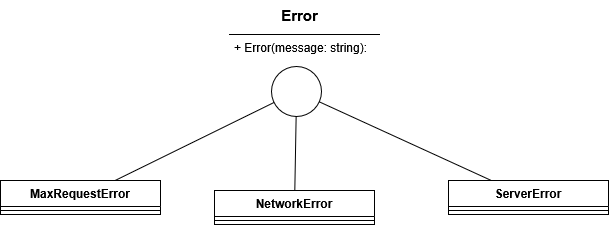
\includegraphics[scale=0.45]{template/images/uml_front/logic/error.png}
    \captionof{figure}{Error}
\end{center}
\textbf{Descrizione del diagramma:}\\
Questo diagramma mostra tutte le classi di errore.
\begin{itemize}
    \item \textbf{MaxRequestError:}
    \begin{itemize}
        \item \textbf{Dipendenze:}
        \begin{itemize}
            \item Error (implementazione): implementa una classe Error personalizzata, derivata da una superclasse Error esistente,
             che include un messaggio specifico per gli errori dovuti al superamento del limite di richieste.
        \end{itemize} 
    \end{itemize}

    \item \textbf{NetworkError:}
    \begin{itemize}
        \item \textbf{Dipendenze:}
        \begin{itemize}
            \item Error (implementazione): implementa una classe Error personalizzata, derivata da una superclasse Error esistente,
            che include un messaggio specifico per gli errori di rete non specifici.
        \end{itemize} 
    \end{itemize}

    \item \textbf{ServerError:}
    \begin{itemize}
        \item \textbf{Dipendenze:}
        \begin{itemize}
            \item Error (implementazione): implementa una classe Error personalizzata, derivata da una superclasse Error esistente,
            che include un messaggio specifico per gli errori di connessione non riuscita al server.
        \end{itemize} 
    \end{itemize}
\end{itemize}

\pagebreak

\paragraph{FilterOptionSlice}
\begin{figure}[h!] \centering
    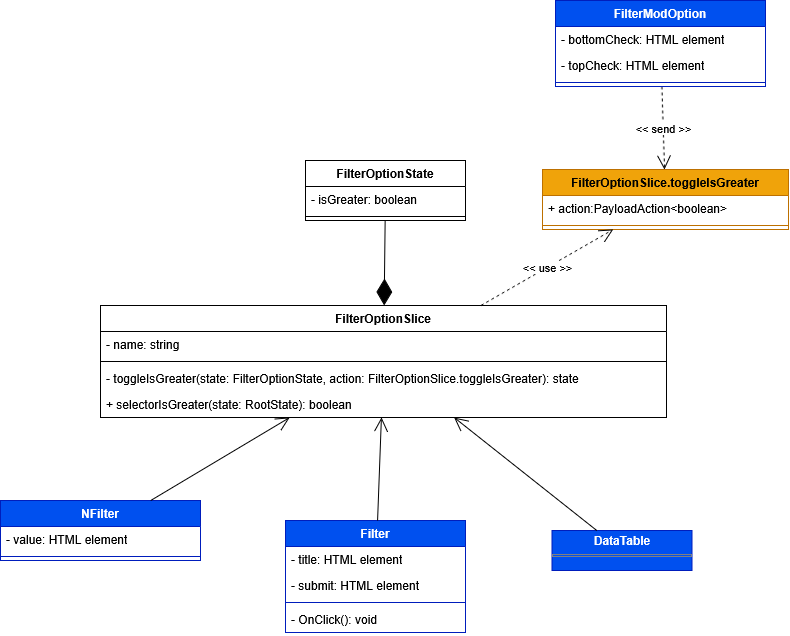
\includegraphics[scale=0.35]{template/images/uml_front/logic/filteroptionslice.png}
    \caption{FilterOptionSlice}
\end{figure}
\textbf{Descrizione del diagramma:}\\
Questo diagramma mostra i componenti per aggiornare e condividere le opzioni di filtraggio.
\begin{itemize}
    \item \textbf{FilterOptionSlice:}
    \begin{itemize}
        \item \textbf{Dipendenze:}
        \begin{itemize}
            \item FilterOptionState (composizione): gestisce la creazione e la distruzione dell'istanza di FilterOptionState, che non è condivisa con altri componenti;
            \item FilterOptionSlice.toggleIsGreater (dipendenza semplice <<use>>): cattura un’istanza di FilterOptionSlice.toggleIsGreater e il reducer imposta il tipo di filtraggio da effettuare utilizzando il payload.
        \end{itemize} 
        \item \textbf{Interazioni:}
        \begin{itemize}
            \item FilterOptionState: viene modificato in base alle action catturate dal reducer della slice.
        \end{itemize} 
        \item \textbf{Action catturate:}
        \begin{itemize}
            \item FilterOptionSlice.toggleIsGreater.
        \end{itemize} 
    \end{itemize}

    \item \textbf{NFilter:}
    \begin{itemize}
        \item \textbf{Dipendenze:}
        \begin{itemize}
            \item FilterOptionSlice (associazione): contiene implicitamente un'istanza di FilterOptionSlice.
        \end{itemize} 
        \item \textbf{Interazioni:}
        \begin{itemize}
            \item FilterOptionSlice: viene utilizzato il metodo selectorIsGreater per reperire le opzioni per il filtraggio.
        \end{itemize} 
    \end{itemize}

    \item \textbf{Filter:}
    \begin{itemize}
        \item \textbf{Dipendenze:}
        \begin{itemize}
            \item FilterOptionSlice (associazione): contiene implicitamente un'istanza di FilterOptionSlice.
        \end{itemize} 
        \item \textbf{Interazioni:}
        \begin{itemize}
            \item FilterOptionSlice: viene utilizzato il metodo selectorIsGreater per reperire le opzioni per il filtraggio.
        \end{itemize} 
    \end{itemize}

    \item \textbf{DataTable:}
    \begin{itemize}
        \item \textbf{Dipendenze:}
        \begin{itemize}
            \item FilterOptionSlice (associazione): contiene implicitamente un'istanza di FilterOptionSlice.
        \end{itemize} 
        \item \textbf{Interazioni:}
        \begin{itemize}
            \item FilterOptionSlice: viene utilizzato il metodo selectorIsGreater per reperire le opzioni per il filtraggio.
        \end{itemize} 
    \end{itemize}

    \item \textbf{FilterModOption:}
    \begin{itemize}
        \item \textbf{Dipendenze:}
        \begin{itemize}
            \item FilterOptionSlice.toggleIsGreater (associazione semplice <<send>>): crea ed emette un’istanza dell’azione FilterOption.toggleIsGreater.
        \end{itemize}
        \item \textbf{Action emesse:}
        \begin{itemize}
            \item FilterOptionSlice.toggleIsGreater.
        \end{itemize}  
    \end{itemize}
\end{itemize}

\paragraph{ViewOptionSlice}
\begin{figure}[h!] \centering
    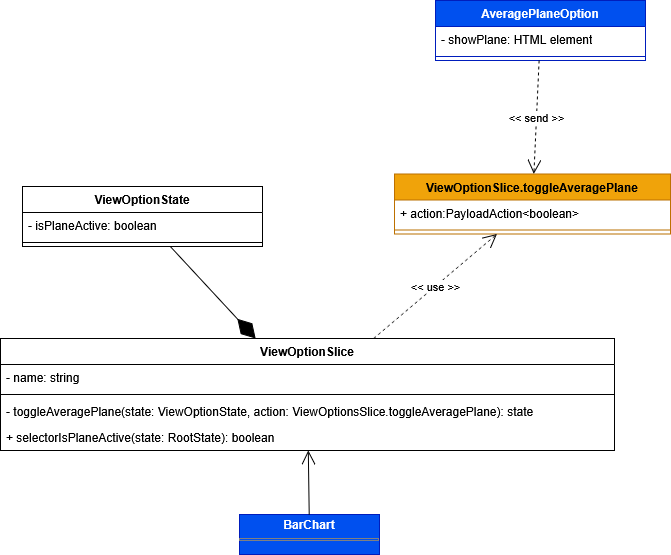
\includegraphics[scale=0.35]{template/images/uml_front/logic/viewoptionslice.png}
    \caption{FilterOptionSlice}
\end{figure}
\textbf{Descrizione del diagramma:}\\
Questo diagramma mostra i componenti per aggiornare e condividere le opzioni di visibilità del piano medio.
\begin{itemize}
    \item \textbf{FilterOptionSlice:}
    \begin{itemize}
        \item \textbf{Dipendenze:}
        \begin{itemize}
            \item ViewOptionState (composizione): gestisce la creazione e la distruzione dell'istanza di FilterOptionState, che non è condivisa con altri componenti;
            \item ViewOptionSlice.toggleAveragePlane (dipendenza semplice <<use>>): cattura un’istanza di ViewOptionSlice.toggleAveragePlane e il reducer imposta la visibilità del piano medio utilizzando il payload;   
        \end{itemize} 
        \item \textbf{Interazioni:}
        \begin{itemize}
            \item ViewOptionState: viene modificato in base alle action catturate dal reducer della slice.
        \end{itemize} 
        \item \textbf{Action catturate:}
        \begin{itemize}
            \item ViewOptionSlice.toggleAveragePlane;
        \end{itemize} 
    \end{itemize}


    \item \textbf{AveragePlaneOption:}
    \begin{itemize}
        \item \textbf{Dipendenze:}
        \begin{itemize}
            \item ViewOptionSlice.toggleAveragePlane (associazione semplice <<send>>): crea ed emette un’istanza dell’azione ViewOptionSlice.toggleAveragePlane.
        \end{itemize}
        \item \textbf{Action emesse:}
        \begin{itemize}
            \item ViewOptionSlice.toggleAveragePlane.
        \end{itemize}  
    \end{itemize}

    \item \textbf{BarChart:}
    \begin{itemize}
        \item \textbf{Dipendenze:}
        \begin{itemize}
            \item ViewOptionSlice (associazione): contiene implicitamente un'istanza di ViewOptionSlice.
        \end{itemize} 
        \item \textbf{Interazioni:}
        \begin{itemize}
            \item ViewOptionSlice: viene utilizzato il metodo selectorIsPlaneActive per reperire le opzioni di visibilità.
        \end{itemize} 
    \end{itemize}

\end{itemize}

\paragraph{RaycastHitSlice}
\begin{figure}[h!] \centering
    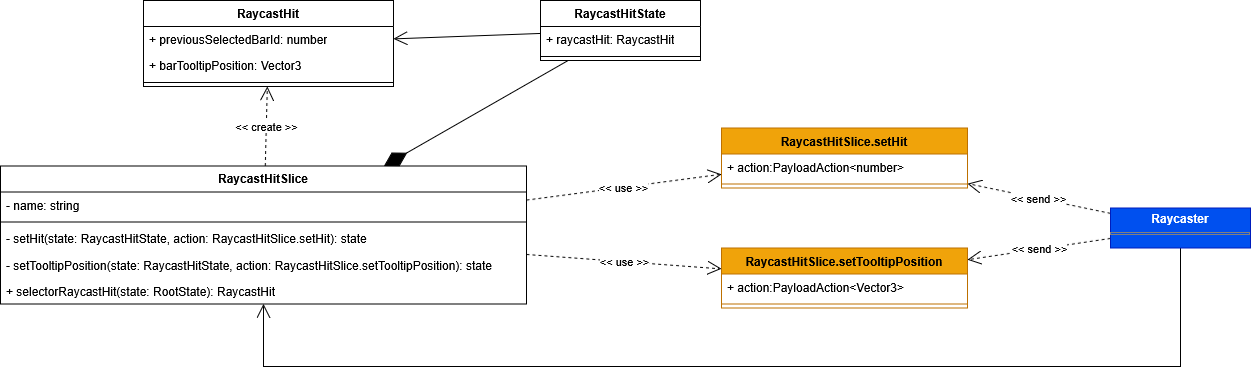
\includegraphics[scale=0.35]{template/images/uml_front/logic/raycastslice.png}
    \caption{RaycastHitSlice}
\end{figure}
\textbf{Descrizione del diagramma:}\\
Questo diagramma mostra i componenti per aggiornare e condividere le informazioni del raycast.
\begin{itemize}
    \item \textbf{RaycastHitSlice:}
    \begin{itemize}
        \item \textbf{Dipendenze:}
        \begin{itemize}
            \item RaycastHitState (composizione): gestisce la creazione e la distruzione dell'istanza di RaycastHitState, che non è condivisa con altri componenti;
            \item RaycastHit (dipendenza semplice <<create>>): responsabile della costruzione del RaycastHit da inserire all’interno del RaycastHitState;
            \item RaycastHitSlice.setHit (dipendenza semplice <<use>>): cattura un’istanza di RaycastHitSlice.setHit e il reducer memorizza la barra del grafico cliccata dall'utente utilizzando il payload;
            \item RaycastHitSlice.setTooltipPosition (dipendenza semplice <<use>>): cattura un’istanza di AppStateSlice.setError e il reducer aggiorna la posizione del tooltip utilizzando il payload.
        \end{itemize} 
        \item \textbf{Interazioni:}
        \begin{itemize}
            \item DataSourceState: viene modificato in base alle action catturate dal reducer della slice.
        \end{itemize} 
        \item \textbf{Action catturate:}
        \begin{itemize}
            \item RaycastHitSlice.setHit;
            \item RaycastHitSlice.setTooltipPosition.
        \end{itemize} 
    \end{itemize}

    
    \item \textbf{RaycastHitState:}
    \begin{itemize}
        \item \textbf{Dipendenze:}
        \begin{itemize}
            \item RaycastHit (associazione): contiene l'oggetto che rappresenta il punto di intersezione tra il cursore del mouse e una barra del grafico.
        \end{itemize} 
    \end{itemize}

    \item \textbf{Raycaster:}
    \begin{itemize}
        \item \textbf{Dipendenze:}
        \begin{itemize}
            \item RaycastHitSlice (associazione): contiene implicitamente un'istanza di RaycastHitSlice;
            \item RaycastHitSlice.setHit (dipendenza semplice <<send>>):  crea ed emette un’istanza dell’azione RaycastHitSlice.setHit;
            \item RaycastHitSlice.setToolTipPosition (dipendenza semplice <<send>>):  crea ed emette un’istanza dell’azione RaycastHitSlice.setToolTipPosition.
        \end{itemize} 
        \item \textbf{Interazioni:}
        \begin{itemize}
            \item RaycastHitSlice: viene utilizzato il metodo selectorRaycastHit per reperire le informazioni del raycast.
        \end{itemize}
        \item \textbf{Action emesse:}
        \begin{itemize}
            \item RaycastHitSlice.setHit;
            \item RaycastHitSlice.setToolTipPosition.
        \end{itemize}   
    \end{itemize}
\end{itemize}

\paragraph{Redux store}
\begin{figure}[h!] \centering
    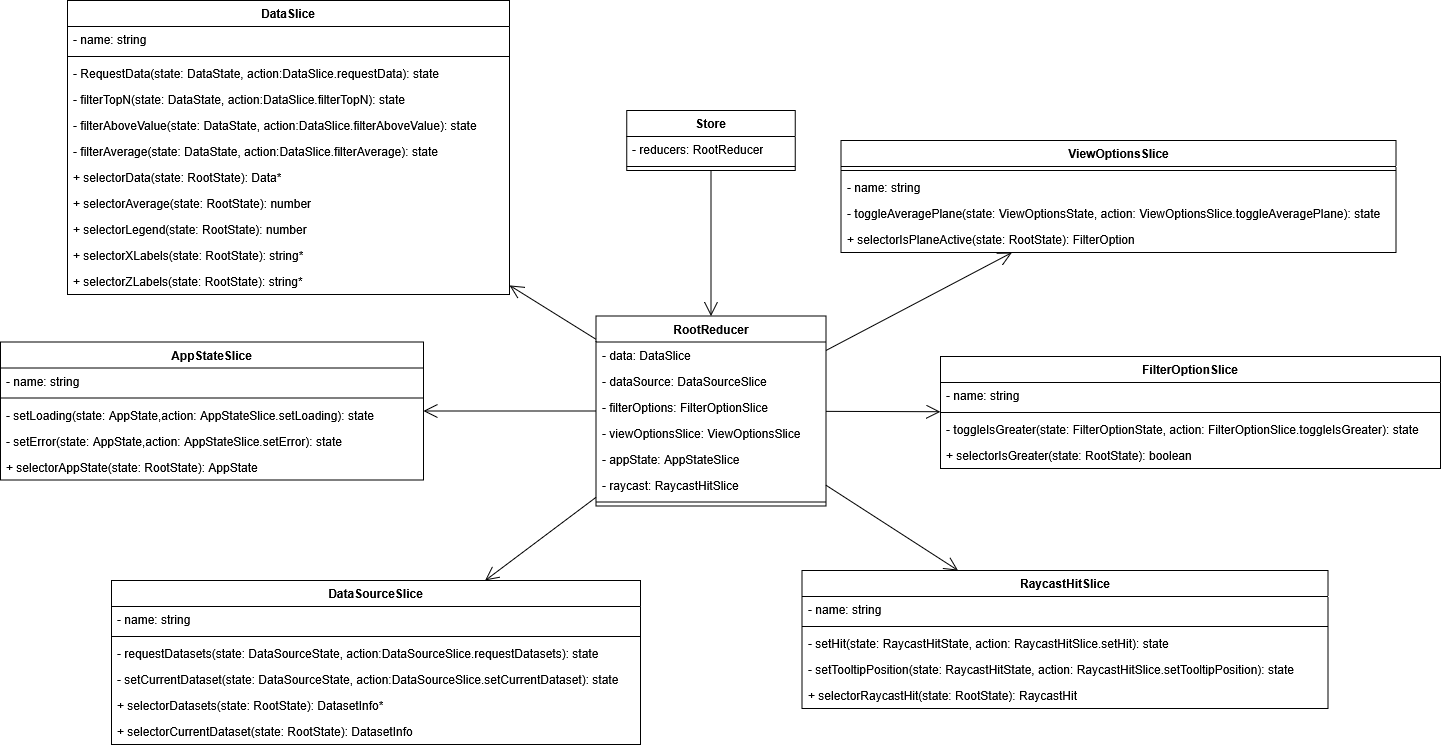
\includegraphics[scale=0.3]{template/images/uml_front/logic/store.png}
    \caption{Redux store}
\end{figure}
\textbf{Descrizione del diagramma:}\\
Questo diagramma mostra lo store e gli slice che compongono lo stato globale dell'applicazione.
\begin{itemize}
    \item \textbf{Store:}
    \begin{itemize}
        \item \textbf{Dipendenze:}
        \begin{itemize}
            \item RootReducer (associazione): possiede un attributo RootReducer che permette di combinare più slice
            con cui lo store interagisce per modificare lo stato globale dell’applicazione.
        \end{itemize}  
    \end{itemize}

    \item \textbf{RootReducer:}
    \begin{itemize}
        \item \textbf{Dipendenze:}
        \begin{itemize}
            \item DataSlice (associazione): possiede un attributo DataSlice per offrire allo store l’accesso alla slice;
            \item DataSourceSlice (associazione): possiede un attributo DataSourceSlice per offrire allo store l’accesso alla slice;
            \item FilterOptionSlice (associazione): possiede un attributo FilterOptionSlice per offrire allo store l’accesso alla slice;
            \item ViewOptionSlice (associazione): possiede un attributo ViewOptionSlice per offrire allo store l’accesso alla slice;
            \item AppStateSlice (associazione): possiede un attributo AppStateSlice per offrire allo store l’accesso alla slice;
            \item RaycastHitSlice (associazione): possiede un attributo RaycastHitSlice per offrire allo store l’accesso alla slice.
        \end{itemize}  
    \end{itemize}
\end{itemize}

\paragraph{Pages}
\begin{figure}[h!] \centering
    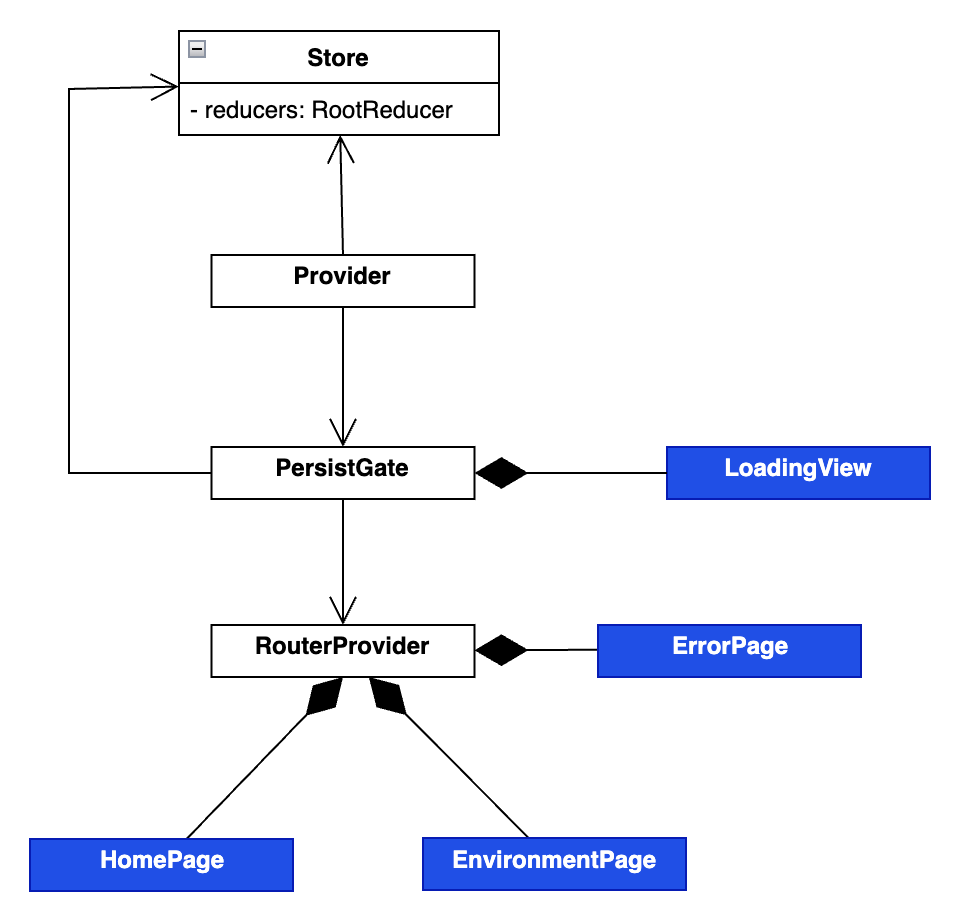
\includegraphics[scale=0.45]{template/images/uml_front/ui/pages.png}
    \caption{Pages}
\end{figure}
\textbf{Descrizione del diagramma:}
Questo diagramma mostra come sono organizzate le varie pagine dell'applicazione.
\begin{itemize}
    \item \textbf{Provider:}
    \begin{itemize}
        \item \textbf{Dipendenze:}
        \begin{itemize}
            \item Store (associazione): utile al Provider di Redux per consentire l'accesso allo store (e quindi allo stato globale) a tutti i componenti nella gerarchia;
            \item RouterProvider (associazione): componente React che gestisce le pagine dell'applicazione e le loro relative rotte.
        \end{itemize} 
    \end{itemize}

    \item \textbf{RouterProvider:}
    \begin{itemize}
        \item \textbf{Dipendenze:}
        \begin{itemize}
            \item HomePage (composizione): componente React che offre all'utente l'interfaccia per la scelta del dataset desiderato;
            \item EnvironmentPage (composizione): componente React che fornisce l'interfaccia per visualizzare un dataset in un ambiente 3D;
            \item ErrorPage (composizione): componente React responsabile della visualizzazione e della gestione degli errori generati dall'applicazione.
        \end{itemize} 
    \end{itemize}

    \item \textbf{HomePage:}
    \begin{itemize}
        \item \textbf{Dipendenze:}
        \begin{itemize}
            \item DatasetItem (composizione): componente React dedicato alla presentazione delle informazioni chiave di un dataset
            \item Footer (composizione): componente React dedicato alla visualizzazione del footer dell'applicazione;
        \end{itemize} 
    \end{itemize}
\end{itemize}

\pagebreak

\paragraph{EnvironmentPage}
\begin{figure}[h!] \centering
    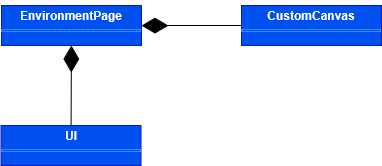
\includegraphics[scale=0.45]{template/images/uml_front/ui/envpage.png}
    \caption{EnvironmentPage}
\end{figure}
\textbf{Descrizione del diagramma:}
Questo diagramma presenta l'organizzazione degli elementi all'interno della pagina dedicata alla visualizzazione di un dataset in ambiente 3D.
\begin{itemize}
    \item \textbf{EnvironmentPage:}
    \begin{itemize}
        \item \textbf{Dipendenze:}
        \begin{itemize}
            \item UI (composizione): componente React che avvolge e gestisce l'intera UI dell'applicazione;
            \item CustomCanvas (composizione): componente React responsabile della visualizzazione e del rendering dell'ambiente 3D.
        \end{itemize} 
    \end{itemize}
\end{itemize}

\paragraph{UI}
\begin{figure}[h!] \centering
    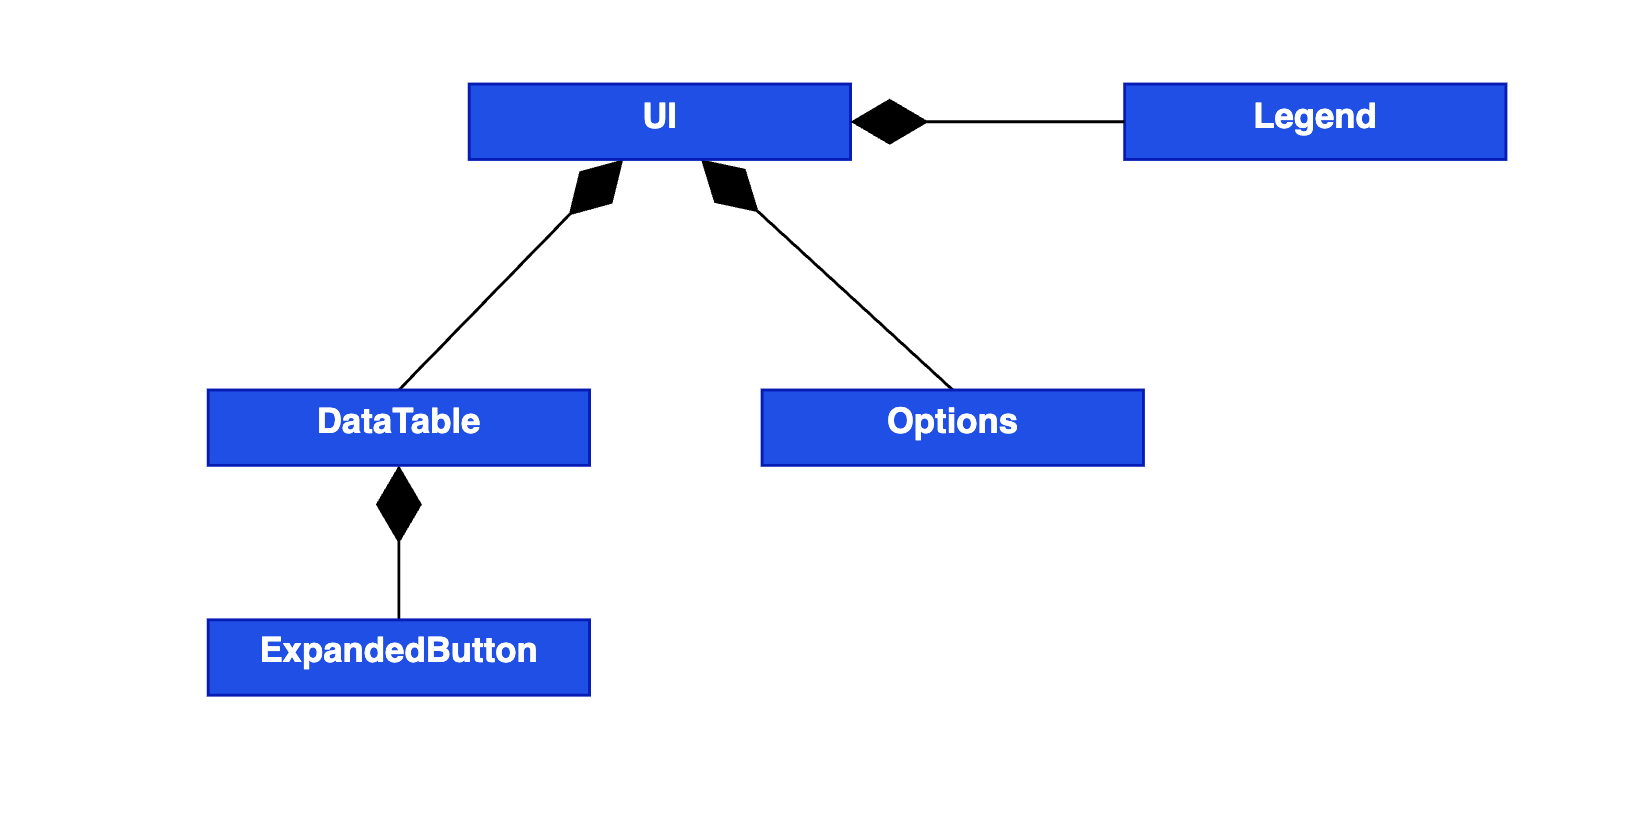
\includegraphics[scale=0.45]{template/images/uml_front/ui/ui.png}
    \caption{UI}
\end{figure}
\textbf{Descrizione del diagramma:}
Questo diagramma presenta la struttura e gli elementi che costituiscono la UI dell'applicazione.
\begin{itemize}
    \item \textbf{UI:}
    \begin{itemize}
        \item \textbf{Dipendenze:}
        \begin{itemize}
            \item Footer (composizione): componente React dedicato alla visualizzazione del footer dell'applicazione;
            \item DataTable (composizione): componente React dedicato alla presentazione di un dataset in formato tabellare;
            \item FilterOptions (composizione): componente React dedicato alla visualizzazione di un form contenente le opzioni per filtrare i dati.
        \end{itemize} 
    \end{itemize}
\end{itemize}

\pagebreak

\paragraph{Options}
\begin{figure}[h!] \centering
    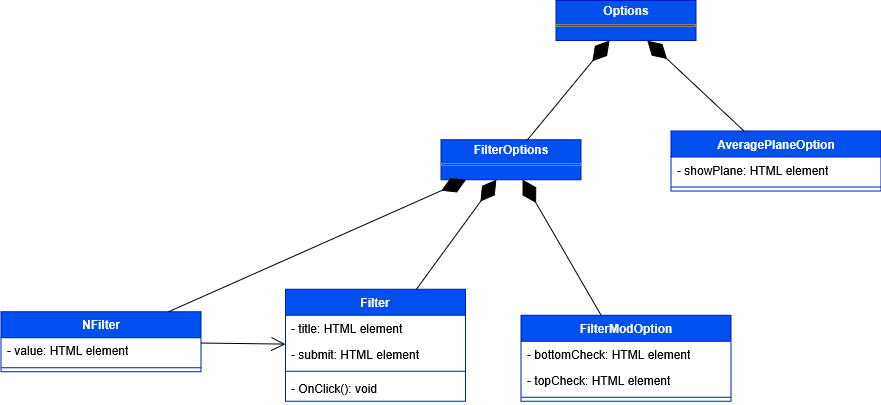
\includegraphics[scale=0.45]{template/images/uml_front/ui/options.png}
    \caption{Filter options}
\end{figure}
\textbf{Descrizione del diagramma:}
Questo diagramma evidenzia la struttura dei gruppi in cui sono suddivise le opzioni di filtraggio e visibilità del piano medio.
\begin{itemize}
    \item \textbf{Option:}
    \begin{itemize}
        \item \textbf{Dipendenze:}
        \begin{itemize}
            \item FilterOptions (composizione): componente React che raggruppa le opzioni di filtraggio;
            \item AveragePlaneOption (composizione): componente React che implementa un filtro generico capace di filtrare valori superiori o inferiori rispetto a un dato valore di riferimento;
        \end{itemize} 
    \end{itemize}

    \item \textbf{FilterOption:}
    \begin{itemize}
        \item \textbf{Dipendenze:}
        \begin{itemize}
            \item NFilter (composizione): componente React che offre la possibilità eseguire un filtraggio sul dataset visualizzando solo i primi N valori più alti o più bassi;
            \item Filter (composizione): componente React che implementa un filtro generico capace di  eseguire un filtraggio visualizzando valori superiori o inferiori rispetto a un dato valore di riferimento;
            \item FilterModOption (composizione): componente React che visualizza un form per permettere all'utente di scegliere se il filtro opererà su valori maggiori o minori;
        \end{itemize} 
    \end{itemize}

    \item \textbf{NFilter:}
    \begin{itemize}
        \item \textbf{Dipendenze:}
        \begin{itemize}
            \item Filter (associazione): componente React che implementa un filtro generico capace di filtrare valori superiori o inferiori rispetto a un dato valore di riferimento.
            In questo caso, è stato esteso per includere un campo che permette di specificare un valore N.
        \end{itemize} 
    \end{itemize}
\end{itemize}

\pagebreak

\paragraph{Custom canvas}
\begin{figure}[h!] \centering
    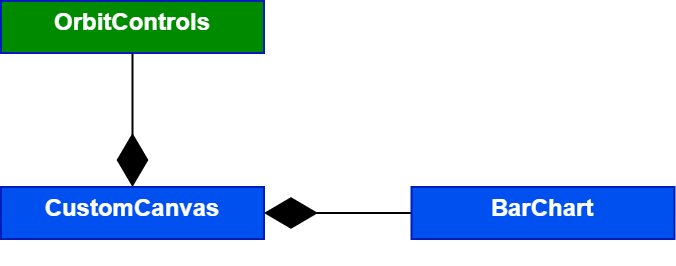
\includegraphics[scale=0.45]{template/images/uml_front/ui/customcanvas.png}
    \caption{Custom canvas}
\end{figure}
\textbf{Descrizione del diagramma:}
Questo diagramma presenta la struttura e gli elementi che costituiscono l'ambiente 3D.
\begin{itemize}
    \item \textbf{CustomCanvas:}
    \begin{itemize}
        \item \textbf{Dipendenze:}
        \begin{itemize}
            \item OrbitControls (composizione): componente React Three Fiber che abilita la navigazione e la manipolazione della telecamera 3D utilizzando gli input del mouse;
            \item BarChart (composizione): componente React che racchiude e gestisce l'intera struttura del grafico 3D.
        \end{itemize} 
    \end{itemize}
\end{itemize}

\paragraph{Bar chart}
\begin{figure}[h!] \centering
    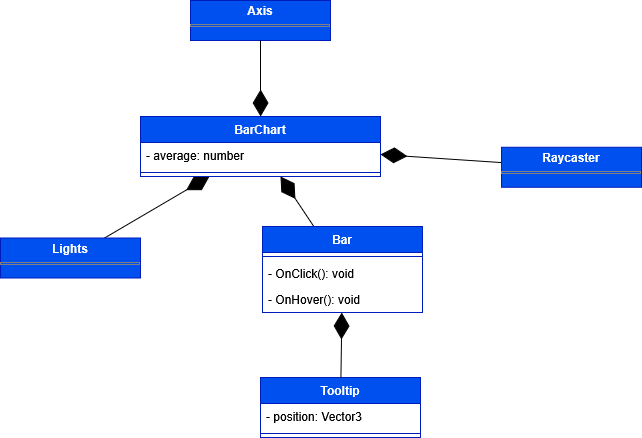
\includegraphics[scale=0.45]{template/images/uml_front/ui/barchart.png}
    \caption{Bar chart}
\end{figure}
\textbf{Descrizione del diagramma:}
Questo diagramma presenta gli elementi che costituiscono il grafico 3D.
\begin{itemize}
    \item \textbf{BarChart:}
    \begin{itemize}
        \item \textbf{Dipendenze:}
        \begin{itemize}
            \item Axis (composizione): componente React che contiene gli assi X, Y e Z del grafico 3D;
            \item AveragePlane (composizione): componente React che permette di visualizzare il piano medio sul grafico 3D;
            \item Lights (composizione): componente React per la gestione delle luci nell'ambiente 3D;
            \item Raycaster (composizione): componente React che implementa la logica per determinare se e dove il cursore del mouse interseca una barra del grafico;
            \item Bars (composizione): componente React dedicato al rendering degli elementi che rappresentano le barre all'interno del grafico 3D.
        \end{itemize} 
    \end{itemize}

    \item \textbf{Bars:}
    \begin{itemize}
        \item \textbf{Dipendenze:}
        \begin{itemize}
            \item Tooltip (composizione): componente React per visualizzare un riquadro informativo al passaggio del mouse sopra la barra del grafico.
        \end{itemize} 
    \end{itemize}
\end{itemize}

\paragraph{Axis}
\begin{figure}[h!] \centering
    
\includegraphics[scale=0.45]{template/images/uml_front/ui/axes.png}
    \caption{Axis}
\end{figure}
\textbf{Descrizione del diagramma:}
Questo diagramma presenta gli elementi che costituiscono ciascuno dei tre assi del grafico 3D.
\begin{itemize}
    \item \textbf{Axis:}
    \begin{itemize}
        \item \textbf{Dipendenze:}
        \begin{itemize}
            \item XAxis (composizione): componente React che rappresenta l'asse X del grafico 3D con relative etichette;
            \item YAxis (composizione): componente React che rappresenta l'asse Y del grafico 3D con relative etichette;
            \item ZAxis (composizione): componente React che rappresenta l'asse Z del grafico 3D con relative etichette.
        \end{itemize} 
    \end{itemize}
\end{itemize}